% =============================================================================
% Stash: paragraphs and figure removed from sec-intro.tex / sec-design.tex
% during the 2026-05-08 restructuring. NOT input from main.tex. Kept here
% so we can move pieces back into the paper if we want them later.
% =============================================================================

% --- Original "Anisotropic data is the realistic case" intro paragraph -------
\textbf{Anisotropic data is the realistic case.}
\looseness -1
Bonnaire's analysis assumes isotropic data: the population covariance
$\Sigmadata = \mathbb{I}$ treats every ambient dimension as carrying
signal of comparable magnitude. This assumption is strongly violated
in the latent-diffusion regime that motivates production systems:
images, video, and molecules concentrate on low-dimensional manifolds
of intrinsic dimension $\dint$ embedded in an ambient latent space
of dimension $\dlat \gg \dint$ \citep{pope2021, brown2022manifold,
stanczuk2024manifold, kamkari2024geometric}. Modern latent-diffusion
architectures \citep{rombach2022highresolution} run diffusion in a
VAE bottleneck whose width is a free design knob set far larger than
$\dint$. Whether---and how---this excess dimensionality affects the
gen-vs-mem transition is a central practical question that the
isotropic theory cannot answer.

% --- Original "Anisotropic data and a four-bulk picture" design paragraph ---
\textbf{Anisotropic data and a four-bulk picture.}
Bonnaire's two-bulk decomposition of the empirical feature
correlation matrix $\Umat$ assumes isotropic data covariance
$\Sigmadata = \mathbb{I}$. In the latent-diffusion regime this
collapses the structure we care about: the data lives on a
$\dint$-dimensional signal manifold inside a $\dlat$-dimensional
ambient space, with population covariance
$\Sigmadata = \diag(\sigsig^2 \mathbb{I}_{\dint},\,
\signoise^2 \mathbb{I}_{\dlat - \dint})$. Empirically (across every
configuration we ran), $\Umat$'s spectrum then splits into
\emph{four} bulks of sizes $\dint$, $\dlat - \dint$, $\nsamp$, and
$\pwidth - \dlat - \nsamp$ (Figure~\ref{fig:overview}), corresponding
to signal, noise-dimension, sample, and rank-null modes.

\begin{figure}[t]
  \centering
  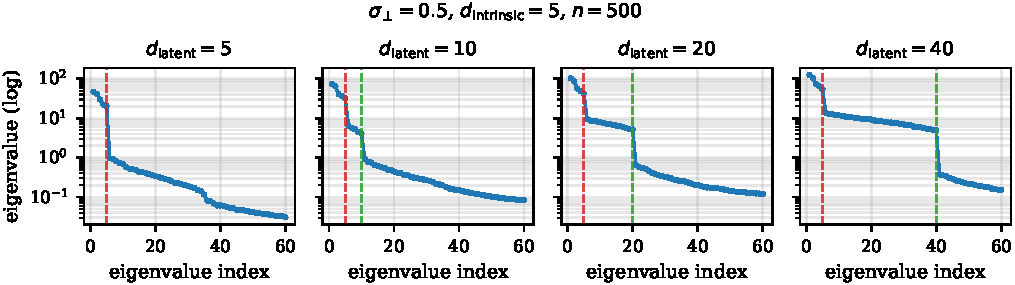
\includegraphics[width=\linewidth]{figures/four_bulk_overview.pdf}
  \caption{\textbf{The four-bulk eigenvalue structure.} Sorted
    log-spectrum of $\Umat$ for an RFNN trained on anisotropic
    Gaussian-mixture data ($\dint = 5$, varying $\dlat$,
    $\nsamp = 500$, $\pwidth = 64\,\dlat$, $\signoise = 0.5$).
    Increasing $\dlat$ inserts a new \emph{noise-dimension bulk}
    between the signal and sample bulks, with cliffs at indices
    $\dint$ (red) and $\dlat$ (green). At $\dlat = \dint$ there is
    no green line and no buffer (the isotropic two-bulk case).}
  \label{fig:overview}
\end{figure}

\textbf{The noise-dimension buffer.}
Each eigenmode $i$ of $\Umat$ is absorbed by the trainable readout
$A$ with characteristic timescale $\tau_i = 1/\lambda_i(\Umat)$, so
the network learns modes in order of decreasing $\lambda_i$. The
new noise-dimension bulk therefore sits temporally \emph{between}
generalization and memorization: every excess latent dimension adds
one mode the network must absorb before reaching the sample bulk
that drives memorization.

% --- Original contributions bullet list from sec-intro.tex -------------------
\textbf{Empirical findings.}
\looseness -1
Our contributions are:
\begin{itemize}\itemsep1pt
\item \textbf{Four-bulk structure (Sec.~\ref{sec:rfnn}).} A new
      noise-dimension bulk of size $\dlat - \dint$ opens in the RFNN
      feature spectrum whenever the data is anisotropic. The
      cumulative-count boundaries land at indices $\dint$ and $\dlat$
      across every configuration we ran, at both $\signoise = 0.01$
      and $\signoise = 0.5$. The signal-to-sample span widens from
      $1.3$ decades at $\dlat = \dint$ to $2.6$ decades at $\dlat =
      200$.
\item \textbf{Buffer mechanism for memorization
      (Sec.~\ref{sec:mlp}).} In a trainable MLP score network with
      hidden width scaled as $h = 8\,\dlat$, $\nsamp = 500$,
      $\taumem$ (memorization fraction first crosses $1\%$) grows
      from $\sim 100\text{k}$ steps at $\dlat = \dint$ to censored at
      ``never within a $300\text{k}$ budget'' for every
      $\dlat / \dint \geq 3$, while $\taugen$ stays in the
      $5$--$15\text{k}$ range until $\dlat$ becomes very large. In
      the RFNN at the same $\nsamp$, $\taumem$ is censored at every
      $\dlat$.
\item \textbf{MLP U-shape at low ambient noise.} At $\signoise =
      0.01$, MLP score error against the analytic mixture score is
      non-monotonic in $\dlat$: it rises sharply from the
      $\dlat = \dint$ baseline, peaks near $\dlat \approx 15$, and
      partially recovers at large $\dlat$ (without dropping below
      baseline at any $\dlat$ we tested). The frozen-feature RFNN
      cannot recover by construction, so this is an MLP-specific
      phenomenon. Our leading hypothesis is sparse, SAE-like
      first-layer features that effectively project onto the
      $\dint$-dimensional signal subspace.
\item \textbf{Practical implication.} For realistic LDMs with
      $\dlat \gg \dint$, the noise-dimension buffer offers
      memorization protection without modifying the loss or
      sacrificing sample quality, and the protection grows with the
      number of excess latent dimensions.
\end{itemize}
